\documentclass{article}

\title{3000 days of Duolingo}
\subtitle{Why eight years with the green owl is enough.}
\date{2025-04-14}
\modified{2025-04-14}

\begin{document}
\section*

\begin{figure}
\center{
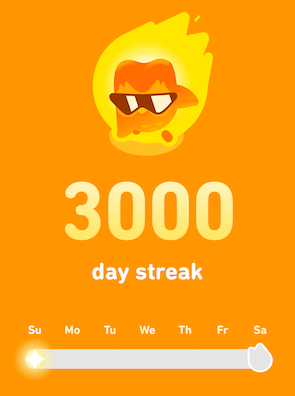
\includegraphics{/images/39-3000-streak.png}
}
\end{figure}

On March 30\sup{th}, 2025, my streak on Duolingo reached 3000 days.
It was also the last day I used the app.
Over the past eight years, I completed the German course at least three times\sidenote{sn-progress-reset}{
 Every time the German course was revised, the app would lose most of my progress.
}, dabbled in French, and breezed through the music and math tracks.
In this article, I share my experience with the app and my motivations for quitting a habit I had for almost a quarter of my life.

\section{why-quit}{Why did I quit}

I'd been using Duolingo since August 2016 as a supplement for my German classes after I moved to Switzerland.
Duolingo helped me drill the language's sentence structure and subtle grammatical aspects.
I had few opportunities to use my German\sidenote{sn-switzerland-german}{
  Swiss people prefer to converse in \href{https://en.wikipedia.org/wiki/Swiss_German}{local dialects} or switch to English.
}; the app allowed me to practice between more traditional lessons.

The app gamifies the learning process, making engaging with the subject more fun.
It encourages you to practice daily in short sections and keep the subject fresh.
However, Duolingo's benefits don't justify the time investment at this point in my learning journey.
There are better ways to improve the skills I care about.

Firstly, Duolingo's gamification has a dark side.
I'm a competitive person, and over time,
I found myself chasing high Duolingo scores,
not pursuing personal educational goals.
Furthermore, I started spending more time with the app than I intended.
For example, Duolingo rewards you with double \textsc{xp}s in the morning if you practice in the evening, and vice versa.
This mechanic encourages you to use the app twice a day: before 12 pm and after 6 pm.
The trick becomes necessary to stay in the ``diamond league'' without wasting an hour a day.
As a result, Duolingo became a gateway for increasing my evening screen time\sidenote{sn-deserve-youtube}{
  Don't I deserve ten minutes on YouTube after being  a good boy and earning 1000\textsc{xp}?
}, which doesn't align with my goals.

Secondly, once you reach a certain level of mastery, Duolingo's exercises become boring and repetitive.
I stopped learning new words or grammar and started going through the motions.
Constructing the same artificial sentences each day became unbearable.

I could learn a new language, but I don't need to.
Learning a language is a massive undertaking that requires a deep emotional investment.
Also, Duolingo isn't a good tool for learning a language from scratch.
Duolingo is like vitamins: it tastes great and won't hurt you,
but the benefits are questionable.

\section{alternatives}{Alternatives}

Duolingo aims to ``develop the best education is the world,''
but the app is not the best way to master any subject.
This section explores alternatives for learning a language, music, and math.

\subsection{alternatives-language}{Language acquisition}

Mastering a language requires obtaining four fundamental skills: reading, listening, speaking, and writing.
These skills have many overlapping components, but you must practice them independently.
For most people, speaking and writing are much harder to improve than reading and listening.
Speaking is the hardest skill to master because it demands semi-automatic reaction:
fluent speech requires thinking in whole phrases and planning, \href{https://en.wikipedia.org/wiki/The_Awful_German_Language}{especially in German}.
With writing, you can always pause, think, and try again without the reader noticing.
Speaking is less forgiving.

If you want to level up your speaking, Duolingo is of little help.
You must go outside your comfort zone and talk to people.
Sign up for a language course.
Check if your community offers free language learner clubs.
If you don't have native speakers around, book time with a teacher on \href{https://www.italki.com}{italki} or \href{https://preply.com}{Preply}.

If you don't feel comfortable talking to people, \href{https://www.pimsleur.com/}{Pimsleur} lessons might unblock you.
The lessons are thirty-minute recordings of plausible conversations with pauses for you to answer prompts out loud.
The recording gives you the correct answer after each pause and moves on.
The main downsides of Pimsleur courses are their price and the need for a space where you feel comfortable saying random phrases out loud.

I felt much more comfortable speaking after completing Pimsleur German lessons.
I attribute this method's success to three factors:
\begin{itemize}
\item You say phrases out loud, practicing the exact skill you want to improve.
\item The pauses after prompts are short, so you must think quickly.
  This constraint imitates the time pressure of a real conversation.
\item You practice pronouncing complete phrases and sentences.
  Using these phrases in a conversation becomes semi-automatic.
\end{itemize}

The next hardest skill to improve is writing.
My friend Ulan came up with an interesting way to practice using LLMs:
he asks ChatGPT to challenge him with a sentence to translate,
provides the translation,
and then asks for feedback.
I love writing by hand, so I use my journal to practice:
each Saturday and Sunday, I record what I did with my family during the day\sidenote{sn-german-log}{
  Only the weekend activity entries are in German.
  The rest of the journal is in English since I use it for work, chores, training progress tracking, and much more.
}.
If I need to write an email in German,
I struggle with it myself and check the grammar in the \href{https://languagetool.org/}{language tool}.

Reading and listening skills are the easiest to level up: consume information in the language you want to learn.
Start by reading books and listening to audiobooks for children and slowly increase the target age\sidenote{sn-books}{
  That's how I found one of my favorite fiction books, \href{https://www.goodreads.com/book/show/68811.Momo}{Momo} by Michael Ende.
}.
If children's books are too hard (I still struggle to translate books to my little kids on the fly at times because of unfamiliar verbs),
try \href{https://www.goodreads.com/book/show/18806935-caf-in-berlin}{André Klein's short stories}.
They are fun and easy to read.
There are also dedicated podcasts for language learners, such as the \href{https://slowgerman.com/}{Slow German} podcast.

\subsection{alternatives-music}{Music}

I've been playing music for twenty years before I started Duolingo's music track,
so I can't judge how well it teaches you the music notation basics.
The note-matching exercises didn't inspire me,
but the sight-reading lessons were pure addiction.

Unfortunately, my piano skills didn't translate well to the on-screen keyboard,
and the on-screen keyboard won't teach you the real instrument.
If you want to learn piano, you must practice at the keyboard.
As of April 2025, the Duolingo music course doesn't support external \textsc{midi} keyboards.

I use \href{https://pianomarvel.com/}{Piano Marvel} to practice sight-reading.
It can also help find easy music to play and practice the music notation.
I also tried \href{https://www.sightreadingfactory.com/}{Sight Reading Factory}, but I didn't like it:
It didn't connect to my piano, and the music it generates is not enjoyable.

\subsection{alternatives-math}{Math}

I studied math at the university and eventually fell in love with the subject.
Math is a vast playground overflowing with toys (geometry, graphs, knots, etc.),
so I expected Duolingo's math course to be fun.
It fell short of my expectations:
it makes you drill second-grade arithmetics, fractions, shape names, and trivial geometric formulas.
Second graders might find valuable insights in that course,
but I wanted to cry from boredom.

The best way to get better at math is to work through math textbook exercises and puzzles.
You can add a social aspect by finding a buddy to challenge you.
During my time at \textsc{dfinity}, I greatly enjoyed exchanging and thinking through math puzzles\sidenote{sn-puzzle-book}{
 Most of these puzzles came from the \href{https://www.goodreads.com/book/show/668035.Mathematical_Puzzles}{Mathematical Puzzles} book by Peter Winkler.
} over lunch with my colleagues.
Exploring puzzles on a whiteboard with smart people made trips to the office much more enjoyable.

I heard good things about \href{https://brilliant.org}{Brilliant}, but I haven't tried it.
It appears to be fun, but I prefer engaging with math using pen and paper (or chalk and a blackboard), not screens.

\end{document}
